 %%
%%
%%   This file is based on the ``apstemplate.tex'' from
%%   the APS files in the REVTeX 4 distribution.
%%   Version 4.1r of REVTeX, August 2010
%%   See the REVTeX 4 README file for restrictions and more information.
%%
%
% This is a template for producing manuscripts for use in PHYS3605 at
% the University of Minnesota
%
% Copy this file to another name and then work on that file.
% That way, you always have this original template file to use.

\documentclass[aps,prstab,reprint,12pt]{revtex4-1}
%\usepackage[title]{appendix}
\usepackage{xspace}
\usepackage{amsfonts}
\usepackage{graphicx}
\usepackage{siunitx}
\usepackage{grffile}
\usepackage{float}
\usepackage{mathrsfs}
\usepackage{physics}

\usepackage[utf8]{inputenc}

\usepackage[letterpaper, margin=0.8in]{geometry}



\providecommand{\units}[1]{\,\ensuremath{\mathrm{#1}}\xspace}


% \newcommand{\appendixpdf}[3]{
%     \includepdf[pages=1,scale=.8,pagecommand={\section{#1}\label{#3}},linktodoc=true]{#2}
%     \includepdf[pages=2-,scale=.8,pagecommand={\section*{Appendix \ref{#3}\quad #1}},linktodoc=true]{#2}
% }

% \linespread{2}

\begin{document}

%Title of paper
\title{A Relation of Mechanical and Electrical Power using a Watt Balance}

% Your name should go first, marked as ``communicating author'' 
\author{M. Laraia}
\thanks{Communicating Author}
% Your lab partner or partners can come next
\author{J. Hirschi}

\affiliation{University of Minnesota, Minneapolis, MN, USA}

\date{\today}

\begin{abstract}
A Watt balance is constructed to measure the relationship between mechanical power and electrical power. The flux through the measurement coil was measured by statically balancing the weight of an object, and while oscillating the balance arm. These two measurements yielded values that were proportional to $0.98 \pm 0.11$.
\end{abstract}

\maketitle

\section{INTRODUCTION}

The International System of units (SI) is being redefined in 2019. In the original system, some of the units were defined in terms of physical objects. The Kilogram, for example, was defined by the International Prototype Kilogram (IPK). The IPK is a block of platinum-iridium alloy forged in 1879 and stored underground in Paris ever since, together with a number of identical sister copies. Every scientific measurement of SI mass is relative to the mass of the IPK. It has been shown, however, that the mass of the IPK and its sister copies has been diverging over time, as shown in figure~\ref{fig:ipk_divergence}. Defining a unit in terms of a physical object is problematic as it cannot be guaranteed that the properties of the object will remain static over long time periods.

For this reason the SI system of units is being redefined to rely only on fundamental constants of the universe. As an example, the meter can be defined in terms of the speed of light in vacuum, and the second can be defined in terms of the frequency of light emitted in a specific energy transition in Caesium-133.
The Kilogram can be defined in terms of Planck's constant, and a device that can measure this relationship is a Watt balance.

\begin{figure}[t]
    \centering
    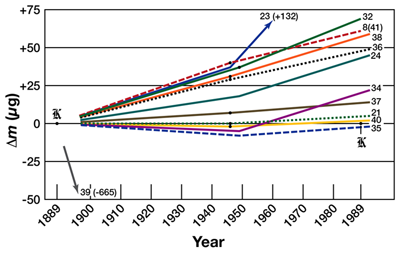
\includegraphics[width=0.95\linewidth]{figs/ipk_mass_drift.png}
    \caption{The mass of the IPK and its sister copies. Evidently the mass of the IPK is diverging from the mass of the copies over time.}
    \label{fig:ipk_divergence}
\end{figure}


What follows is a general description of how a Watt balance works. A more detailed description will follow in Section~\ref{s:theory} and Section~\ref{s:device}.
A watt balance resembles an equal arm balance with each side of the arm having a permanent magnet hanging over coiled wire. The Watt balance is operated in two modes. In the first mode an object is placed on the balance, and a current applied to one coil creates a force on the adjacent permanent magnet that acts against the weight of the object. In the second mode one of the coils is driven to oscillate the balance arm. The motion of the permanent magnet in the second coil induces an electromotive force that can be measured. The two modes are called the force mode and the velocity mode.


Planck's constant can be recovered when measuring induced emf in the velocity mode and the applied current in the velocity mode. The induced emf can be measured with Josephson junctions, and the applied current in the force mode can be measured with a Josephson junction measuring the voltage over a quantum Hall resistance standard. This is discussed further at the end of Section~\ref{s:theory}.

The official Watt balance at the National Institute of Standards and Technology was built with Josephson junctions and quantum Hall resistance standards. To redefine the SI kilogram, the Watt balance was used with a standard mass calibrated to the IPK to fix Planck's constant relative to the kilogram. After redefinition, a Watt balance could be used to precisely measure the mass of a standard mass in terms of Planck's constant.

This provides the motivation for building a Watt balance. As we do not have access to Josephson junctions and quantum Hall resistance standards for this experiment, the device and the experiment described here will not measure the relationship to Planck's constant. Instead we aim to build a Watt balance that can relate the mechanical and electrical power in the two modes described above.

\begin{figure}
    \centering
    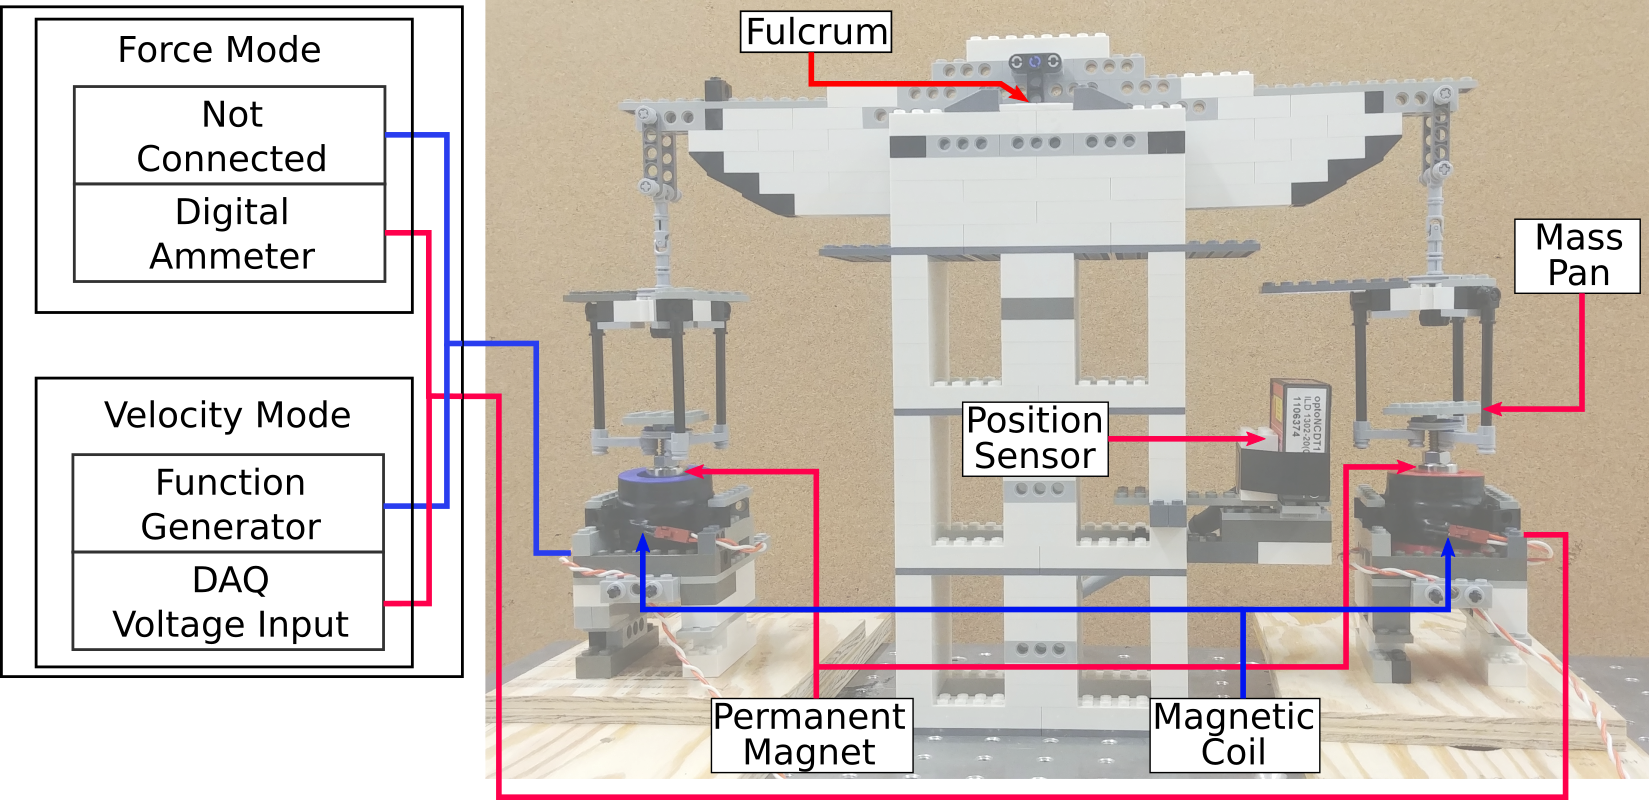
\includegraphics[width=0.95\linewidth]{figs/watt_balance.png}
    \caption{An image of the completed device used in this experiment.}
    \label{fig:device_image}
\end{figure}


\section{THEORY}\label{s:theory}

A Watt balance operates by balancing an electromagnetic force with a mechanical force. This can be done by operating the Watt balance in two modes. In the velocity mode one coil is driven to create oscillating motion in the arm while the other coil uses Faradays law to measure an induced electro-motive force $\mathscr{E}$. In the force mode only one coil is operated to provide a force which balances the gravitational force acting on a mass. As mentioned earlier, the velocity mode is a pseudo-calibration step, which will be described in further detail in this section.

Faraday's Law states that when a permanent magnet moves near a looped wire, an emf $\mathscr{E}$ is produced, which induces a voltage in the wire proportional to the number of loops $N$ and the rate of change of the magnetic flux $\Phi_B$
\begin{equation}\label{eq:Faraday}
\mathscr{E} =-N\frac{d \Phi_B^N}{dt}.
\end{equation}

If we assume that the rate of change of the magnetic flux is proportional to the velocity of the permanent magnet, then we can rewrite this equation as follows, where $\Phi_v = (\Phi_B^NN)_v$:
\begin{equation}\label{eq:velocity_equation}
    \Phi_v  = \frac{V}{v}
\end{equation}

When the balance arm is driven in the velocity mode, a voltage is induced proportional to the magnetic flux $\Phi_v$ and the velocity of the arm. A schematic diagram of the velocity mode is shown in figure~\ref{fig:vmode-concept}. This measurement can be used to factor out the flux $\Phi_f$ in the force mode, as will be described below.

\begin{figure}[b]
    \centering
    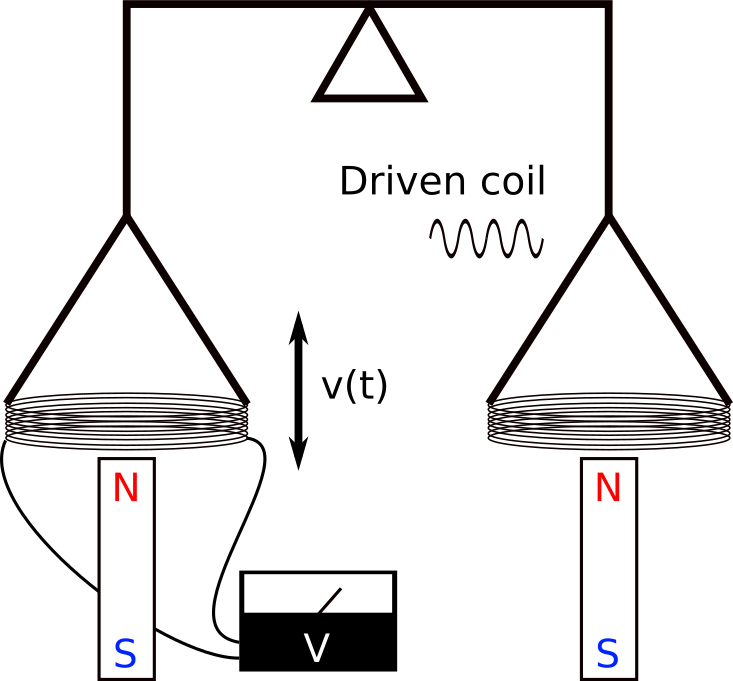
\includegraphics[width=0.6\linewidth]{figs/watt-balance-vmode.png}
    \caption{Conceptual diagram of the velocity mode. The coil on the right is driven sinusoidally with an electromagnet. The coil is thereby driven to oscillate near a permanent magnet, inducing an emf in the coil.}
    \label{fig:vmode-concept}
\end{figure}

The Lorentz force law can be described as follows, where $q$ is a charge, $v$ is its velocity, $E$ is the electric field, and $B$ is the magnetic field:
\begin{equation}
    \vec{F} = q(\vec{E}+v\times \vec{B})
\end{equation}

We can drop the electric field term because the latent electric field is negligible compared to the magnetic field. Expressing the second term in terms of the current $I$ through a length of wire $l$ yields the following:
\begin{equation}
    \vec{F} = I \vec{l}\times \vec{B}
\end{equation}

If the wire is instead looped, then we can integrate this equation over the length of the loop as follows to get a force in the direction normal to the plane of the loop $\hat{n}$:
\begin{equation}
    \vec{F} = I\int\vec{dl}\times\vec{B}  = (\Phi_B^N N)_fI \hat{n}
\end{equation}

In the force mode the Watt balance will be operated to generate a force counteracting the gravitational force on a mass $m$. This produces the following relationship, where $\Phi_f = (\Phi_B^NN)_f$
\begin{equation}\label{eq:force_equation}
    \Phi_f = \frac{mg}{I}
\end{equation}
where $g$ is the local acceleration due to gravity. A schematic diagram of the force mode is shown in figure~\ref{fig:fmode-concept}.

% \begin{figure}[t]
%      \centering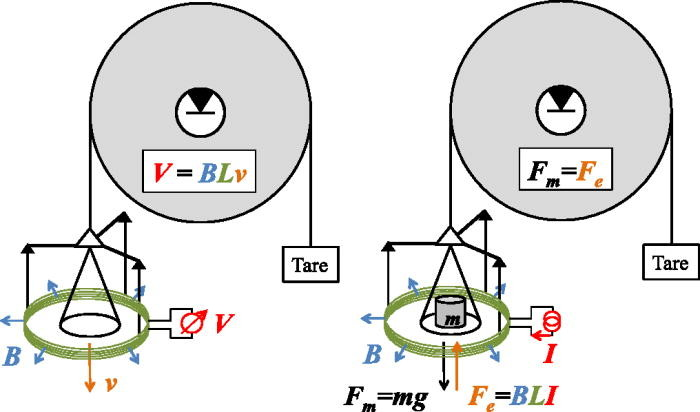
\includegraphics[width=.95\linewidth]{figs/Force_Diagram.jpeg}
%      \caption{Velocity mode measurement, illustrated on the left, depicts a coil moving vertically in a radial magnetic field and a voltage $V$ is induced. Force mode measurement, right, displays that the upward electromagnetic force generated by the coil opposes the gravitational force exerted on the mass. \cite{Chao2015}}\label{fig:Force}
% \end{figure}


\begin{figure}[b]
    \centering
    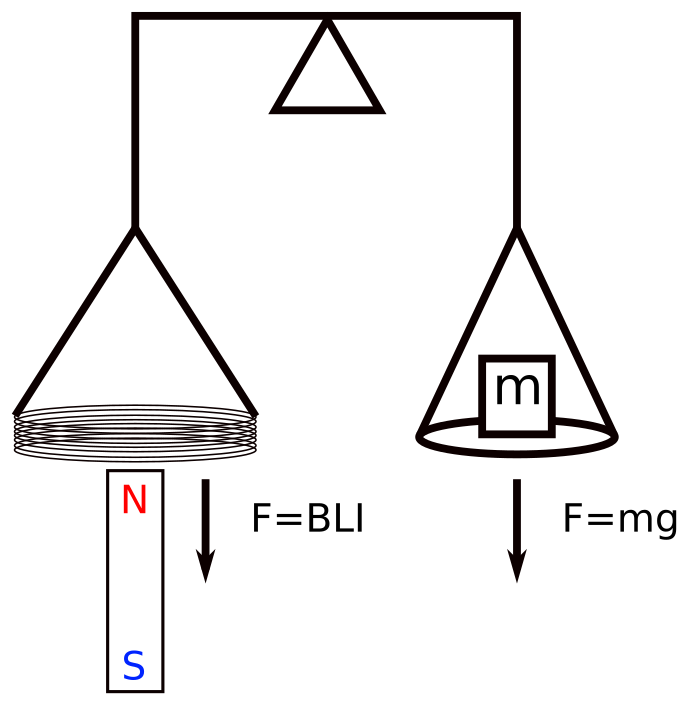
\includegraphics[width=0.6\linewidth]{figs/watt-balance-fmode.png}
    \caption{Conceptual diagram of the force mode. A mass is placed on the platform, while a current is applied to one of the coils. This creates a magnetic force that balances the weight of the mass.}
    \label{fig:fmode-concept}
\end{figure}

Assuming that $\Phi$ remains constant between measurements in the velocity and force modes, equations~\ref{eq:velocity_equation} and~\ref{eq:force_equation} can be used to factor out the $\Phi$ term. This is important because the flux $\Phi$ is very difficult to measure directly. Furthermore, any linear correction factors that would normally have to be considered in such a setup can be accounted for in the same way as $\Phi$. We expect these factors to be present and equal in both modes of operation and can therefore be rolled in with $\Phi$. Possible linear correction factors of this sort include the moment of inertia of the balance arm and various linear sources of friction. We arrive at the following equation
\begin{equation}\label{eq:watt_equation}
    \frac{\Phi_f}{\Phi_v} = \frac{VI}{mgv} = 1
\end{equation}

Equation~\ref{eq:watt_equation} relates mechanical power $mgv$ to electrical power $VI$. In our experiment we will measure $V$, $I$, and $v$, assuming $m$ and $g$ are known.

A successful experiment would measure a 1-to-1 correspondence between electrical and mechanical power, confirming equation~\ref{eq:watt_equation}. If successful, the watt balance we build could be used to measure other quantities. For example, if the mass of an object is known equation~\ref{eq:watt_equation} can be used to measure the local gravitational acceleration. Conversely, if the local gravity is known we can measure the mass of an unknown object.

Finally, we provide an additional discussion on the quantum effects used in the official NIST Watt balance. 
The Josephson effect is an effect in the quantum realm describing current across a Josephson function. A Josephson junction consists of two superconductors coupled by a weak link.\ 
When an electric field oscillating at a microwave frequency $f$ is applied a small current is forced through the junction. This creates a quantized voltage across the junction.
Many Josephson junctions can be combined to create a voltage standard that couples the generated voltage to Planck's constant as follows, where $h$ is Planck's constant, $e$ is the charge of an electron, and $K_J$ is Josephson constant
\begin{equation}\label{eq:josephson}
    V=\frac{h}{2e}f \equiv \frac{1}{K_J} f
\end{equation}
The NIST Watt balance uses 250,000 junctions to measure any voltage up to 10\si{V} with a precision of 1\si{nV}. The approximate \$100,000 cost of this setup makes it unfeasable in an MXP classroom setting~\cite{Chao2015}.
\newpage

The quantum Hall effect is a special case of the classical Hall effect, but where the Hall conductance is quantized. This effect occurs in two-dimensional systems of electrons subjected to low temperatures and strong magnetic fields. The quantized Hall conductance $\sigma$ can be described as follows, where $\nu$ belongs to either the set of integers or to a set of known fractions
\begin{equation}
    \sigma = \frac{I}{V_\mathrm{Hall}} = \nu \frac{e^2}{h}
\end{equation}

If we consider only the integer Hall conductance, then we arrive at the following quantized Hall resistance $R_H$, where $R_K$ is the von Klitzing constant
\begin{equation}\label{eq:resistance}
    R_H=\frac{V_H}{I}=\frac{1}{\nu}\frac{h}{e^2} \equiv \frac{1}{\nu} R_K
\end{equation}

The NIST Watt balance uses the quantum Hall effect to measure resistance with a relative uncertainty of 1 in $10^9$. Together with a Josephson voltage standard this can be used to measure current with incredible precision. To determine the value of $VI$ from equation~\ref{eq:watt_equation}, we combine two Josephson standards from equation~\ref{eq:josephson} and a Hall resistance standard from equation~\ref{eq:resistance} to yield the following expression, where $C$ is a known constant related to the number of Josephson junctions
\begin{equation}
    VI=V \frac{V_H}{R_H} = C f_1 f_2 {\left(\frac{h}{2e}\right)}^2 \frac{e^2}{h}=C \frac{f_1f_2}{4} h
\end{equation}

We see that $h$ finally drops out, and plugging back into equation~\ref{eq:watt_equation} yields the following expression
\begin{equation}\label{eq:planck}
    C \frac{f_1f_2}{4} h = mgv
\end{equation}

Equation~\ref{eq:planck} defines the kilogram in terms of Planck's constant and other measurements in units defined by other fundamental constants of the universe. This is the desired result.




%%%%%%%%%%%%%%%%%%%%%%%%%%%%%%%%%%%%%%%%%%%%%%%%%%%%%%
%%%%%%%%%%%%%%%%%%%%%%%%%%%%%%%%%%%%%%%%%%%%%%%%%%%%%%
\section{EXPERIMENTAL SETUP}\label{s:device} %%%%%%%%
%%%%%%%%%%%%%%%%%%%%%%%%%%%%%%%%%%%%%%%%%%%%%%%%%%%%%%
%%%%%%%%%%%%%%%%%%%%%%%%%%%%%%%%%%%%%%%%%%%%%%%%%%%%%%

\begin{figure}[t]
    \centering
    \includegraphics[width=0.8\linewidth]{figs/device-diagram.png}
    \caption{Schematic diagram of the device. The two coils are labeled blue and red to avoid confusion. The blue coil is driven in the velocity mode. A current is applied to the red coil in the force mode, and the induced emf is measured in the velocity mode.}
    \label{fig:device_diagram}
\end{figure}


In this section we describe the device construction. An image of the completed design is shown above in figure~\ref{fig:device_image}. A diagram of the experimental setup is shown in figure~\ref{fig:device_diagram}.
LEGO bricks were chosen to build this device as it is easy not only to quickly build a prototype, but also to make modifications to the prototype along the way. An arm balances on a central tower.
From each end of the arm hangs a platform. A universal joint is used to hang the platform from the arm to allow the platform to hang freely. From each platform hang a pair of permanent neodymium magnets.
The magnets are oriented antiparallel in a quadrupolar configuration. Below each pair of magnets is a 3D-printed cylinder that carries the coiled wire.
The cylinder is designed with a groove to hold the wire. 3,000 turns of 36-AWG magnetic wire are wound onto each cylinder.

The two coils are labeled as the red coil and the blue coil to limit confusion, as shown in figure~\ref{fig:device_diagram}. In the velocity mode, the blue coil is connected to an HP Agilent 33120A arbitrary waveform generator (function generator). The red coil is connected to an NI 6321 data acquisition (DAQ) card to measure the induced voltage. In the force mode the blue coil is disconnected. The red coil is connected in series to an SRS600 low noise preamplifier and an HP 34410A digital multimeter configured to measure current. The SRS600 output is controlled by the DAQ card.

A previous design had the permanent magnets mounted on the base and the coils suspended from the platforms. The configuration described here has the coils mounted on the base and the magnets suspended from the platforms. This configuration was chosen as the wires to the coils suspended from the platform were too rigid to allow the platform to hang freely as the arm moved. The drawback to the configuration with the suspended magnets is that as each magnet weighs on the order of 100g,
, the moment of inertia of the arm is increased significantly.


A MicroEpsilon laser triangulation displacement sensor is mounted below one of the platforms. This sensor is sensitive to within 1\si{\mu m} within a measurement range of 30-50\si{mm}. The top of the platform stage is extended with a flat LEGO brick to reflect the displacement sensor laser. A piece of white printer paper is attached below this extension to ensure the shape of the LEGO brick does not distort the reflection of the laser. The displacement sensor is connected to the measurement computer with an RS232 serial interface.


%%%%%%%%%%%%%%%%%%%%%%%%%%%%%%%%%%%%%%%%%%%%%%%%%%%%%%
%%%%%%%%%%%%%%%%%%%%%%%%%%%%%%%%%%%%%%%%%%%%%%%%%%%%%%
\section{PROCEDURE}
%%%%%%%%%%%%%%%%%%%%%%%%%%%%%%%%%%%%%%%%%%%%%%%%%%%%%%
%%%%%%%%%%%%%%%%%%%%%%%%%%%%%%%%%%%%%%%%%%%%%%%%%%%%%%


In this section we describe the data acquisition process. In the first stage the emf induced in the loop is measured as a function of the velocity of the balance arm. In the second stage the current required to balance the arm is measured for a given mass configuration. We begin by describing the data acquisition process for the velocity mode. % definitely need a TODO

The displacement data is gathered from the MicroEpsilon displacement sensor with a LabView program. The LabView program runs at a fixed 100Hz frequency, while the measurement rate of the displacement sensor is 750Hz \cite{muepsilon_manual}. To compensate for this difference the measurements collected at each time step are averaged. An added benefit is that this smooths the noisy signal from the displacement sensor.

%%%%%%%%%%%%%%%%%%%%%%%%%%%%%%%%%%%%%%%%%%%%%%%%%%%%%%
%%%%%%%%%%%%%%%%%%%%%%%%%%%%%%%%%%%%%%%%%%%%%%%%%%%%%%
\subsection{VELOCITY MODE}
%%%%%%%%%%%%%%%%%%%%%%%%%%%%%%%%%%%%%%%%%%%%%%%%%%%%%%
%%%%%%%%%%%%%%%%%%%%%%%%%%%%%%%%%%%%%%%%%%%%%%%%%%%%%%

In the velocity mode the blue coil is driven with the function generator while the induced voltage in the red coil is measured with the DAQ. The function generator used in this experiment has a lower signal amplitude limit of 50\si{mV_{pp}}.
To further reduce the signal amplitude the red coil is separated from the function generator output with a 1:10 voltage divider circuit.

During a measurement run the function generator was configured to output a signal with an amplitude range of $50-300$ \si{mV_{pp}} and a frequency range of $100-1000$ \si{mHz}. This frequency range was chosen to be close to the natural frequency of the balance arm, which was determined to be roughly in the range $550-650$ \si{mHz}. The signal amplitude for a particular measurement run and frequency were chosen such that the measured peak-to-peak displacement was approximately 1\si{mm}. The LabView program was configured to collect data with a 10ms time step.

%%%%%%%%%%%%%%%%%%%%%%%%%%%%%%%%%%%%%%%%%%%%%%%%%%%%%%
%%%%%%%%%%%%%%%%%%%%%%%%%%%%%%%%%%%%%%%%%%%%%%%%%%%%%%
\newpage\subsection{FORCE MODE}
%%%%%%%%%%%%%%%%%%%%%%%%%%%%%%%%%%%%%%%%%%%%%%%%%%%%%%
%%%%%%%%%%%%%%%%%%%%%%%%%%%%%%%%%%%%%%%%%%%%%%%%%%%%%%

In the force mode a current is applied to the red coil to oppose the weight of a mass placed in the platform. A LabView program controls the current output to the red coil using a PID controller. A PID controller is a control-loop feedback mechanism to continuously modulate an output to move the system to a desired state.
The PID calculates the error between the desired input (setpoint) and the measured process variable.
The PID calculates a correction with three terms, the proportional, the integral, and the differential terms. At each time step the proportional term considers the current value of the error, the integral term considers how long the error has persisted, and the differential term considers how the error changes over time.
More information about PID theory can be found in \cite{pid}.

The magnitude of the proportional, integral, and differential corrections is determined by the paramters $K_p$, $K_I$, and $K_d$. The values for these constants were determined through trial and error. The PID was run with an arbitrary mass on the balance.
The parameters were tuned first by adjusting $K_p$ and $K_I$ until the balance was able to slowly bring the process variable near the set point.
Then the $K_d$ term was increased until the PID was able to counter small oscillations about the set point. The parameters were accepted when the balance was able to go start from rest and remain within 1\% of the setpoint for more than 5 seconds. The values for the parameters are summarized in table~\ref{tab:pid}. The setpoint was determined by placing a level over the center of the balancing arm and varying the setpoint until the balance arm was level. Using this method the setpoint was chosen as 8.5mm.

\begin{table}[b]
    \centering
    \begin{tabular}{|c|c|c|}\hline
        $K_p$ & $K_I$ & $K_d$ \\\hline
        0.1 & 0.01 & 0.005 \\\hline
    \end{tabular}
    \caption{Tuned parameters for the PID controller. These parameters are used to operate the Watt balance for the force mode measurement.}
    \label{tab:pid}
\end{table}

Two current measurements are made when making a force mode measurement. In the first step the current required to balance a tare mass is recorded. The mass of the tare mass does not need to be known, as will be shown in a moment. In the second step a known mass is placed on the opposite coil, and the current required to balance both masses is recorded. 
\begin{align}
    I_T \Phi_f &= -m_T g ,\quad I \Phi_f = (m-m_T)g \nonumber \\
    \Phi_f &= \frac{mg}{I-I_T} \label{eq:force_current}
\end{align}
As equation~\ref{eq:force_current} shows, the tare mass is irrelevant. It is possible that the current required to balance the mass will drift. To correct for the drift these steps are repeated 2-3 times for a given measurement run. The resulting measurements with and without the mass are averaged to get $I_T$ and $I$.

The mass of a given object was determined with a chemical scale accurate to 1mg. The mass was varied in small increments by bundling small amounts of wire. The tare mass used was typically a 2g calibrated mass. The resulting measurements are shown in figure~\ref{fig:force-data}, and will be discussed further in section~\ref{s:discussion}.

%This measurement involves placing a known mass onto the mass pan, located above coil A in figure \ref{fig:chao_balance}, and inducing an electromagnetic force on coil B to counteract the gravitational force of the mass. The magnitude of the electromagnetic force will be controlled in a way such that the balance arm will stay in it's nulled position after masses are added or removed. A proportional integral derivative controller (PID), programmed using LabVIEW, will be used to regulate the electromagnetic force. This type of controller uses manual feedback to automate the changes necessary in the
%electromagnetic force to hold the balance in the null position. Several constants will need to be determined and inputted into the PID controller to regulate this specific system.

%The measurement process will involve measuring the current needed to balance a tare mass and a calibrated mass. We can then relate the two measurements to solve for the $(\Phi_B N)_F$ factor. However, to cancel out any drift that may occur in our measurements of current the measurement process will be repeated multiple times with the same masses. This will improve the accuracy of calculated $(\Phi_B N)_F$ factor. In order to calculate the flux integral from force mode, we need to know the local gravitational constant $g$ which can be referenced from the National Oceanic and Atmospheric Administration.

% \subsection{Relation of Mechanical and Electrical Power}

% If successful, our watt balance will measure a 1-to-1 correspondence between $(\Phi_B N)_v$ and $(\Phi_B N)_F$. 


%%%%%%%%%%%%%%%%%%%%%%%%%%%%%%%%%%%%%%%%%%%%%%%%%%%%%%
%%%%%%%%%%%%%%%%%%%%%%%%%%%%%%%%%%%%%%%%%%%%%%%%%%%%%%
\section{DATA ANALYSIS}\label{s:discussion}
%%%%%%%%%%%%%%%%%%%%%%%%%%%%%%%%%%%%%%%%%%%%%%%%%%%%%%
%%%%%%%%%%%%%%%%%%%%%%%%%%%%%%%%%%%%%%%%%%%%%%%%%%%%%%


%%%%%%%%%%%%%%%%%%%%%%%%%%%%%%%%%%%%%%%%%%%%%%%%%%%%%%
%%%%%%%%%%%%%%%%%%%%%%%%%%%%%%%%%%%%%%%%%%%%%%%%%%%%%%
% Force Mode %%%%%%%%%%%%%%%%%%%%%%%%%%%%%%%%%%%%%%%%%
%%%%%%%%%%%%%%%%%%%%%%%%%%%%%%%%%%%%%%%%%%%%%%%%%%%%%%
%%%%%%%%%%%%%%%%%%%%%%%%%%%%%%%%%%%%%%%%%%%%%%%%%%%%%%

In this section we describe the steps used to process and analyze the measured data. The general formula for propagasub
The error propagation for a multi-variable function $\gamma$ defined for $n$ variables $\delta_1\cdots\delta_n$ is defined as follows
\begin{equation}
    \sigma_\gamma^2 = \sum_{\delta_1}^{\delta_n} \sigma_\delta^2 {\left( \frac{\partial \gamma}{\partial \delta} \right)}^2
\end{equation}
All uncertainties quoted in this analysis are calculated using this formula.

For the force mode we made at least two measurements each of $I_T$ and $I$. We calculate each current as the mean of these measurements, and the uncertainty as the sample standard deviation. If the standard deviation is less than 0.01mA then this value is used instead.

The resulting force measurements are shown in figure~\ref{fig:force-data}a. A linear least squares regression was performed on the mass vs current data. The reduced $\chi^2$ value for the fit was 1.35, which suggests the fit is good.

\begin{figure}[b]
    \centering
    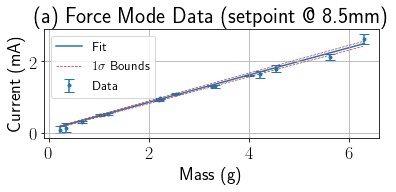
\includegraphics[width=\linewidth]{figs/data/force_data.png}
    \caption{Force mode measurements, and the least squres regression. The fit parameters suggest $\Phi_f=25.55 \pm 0.51\si{\frac{kgm}{s^2A}}$. The reduced $\chi^2$ value is 1.35, suggesting a good fit.}
    \label{fig:force-data}
\end{figure}


The local gravity can be estimated using a tool provided by the National Oceanic and Atmospheric Administration (NOAA) for a given geographic location. Using this tool and the coordinates of the lab (44.975224 N, 93.234298 W, 830ft above sea level) the local gravity is estimated as $g=980585\pm2\mathrm{milligal}$. Using equation~\ref{eq:force_current} the factor $\Phi_f$ can be extracted from the slope of figure~\ref{fig:force-data}a and this value for gravity. The value of $\Phi_f$ is determined to be $25.55 \pm 0.51\si{\frac{kgm}{s^2A}}$

% \begin{figure}[t]
%     \centering
%     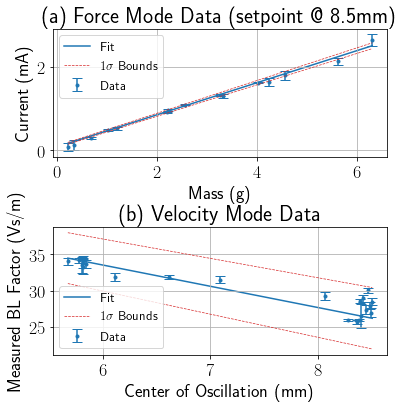
\includegraphics[width=\linewidth]{figs/data/final_data.png}
%     \caption{The }
%     \label{fig:both-data}
% \end{figure}

%%%%%%%%%%%%%%%%%%%%%%%%%%%%%%%%%%%%%%%%%%%%%%%%%%%%%%
%%%%%%%%%%%%%%%%%%%%%%%%%%%%%%%%%%%%%%%%%%%%%%%%%%%%%%
% Velocity Mode %%%%%%%%%%%%%%%%%%%%%%%%%%%%%%%%%%%%%%
%%%%%%%%%%%%%%%%%%%%%%%%%%%%%%%%%%%%%%%%%%%%%%%%%%%%%%
%%%%%%%%%%%%%%%%%%%%%%%%%%%%%%%%%%%%%%%%%%%%%%%%%%%%%%


Calculating the $\Phi_v$ term for the velocity mode has a few additional steps. The first problem arises when trying to calculate the time derivative of the displacement data. One method to calculate the derivative of a signal is the centered difference method (CD), a variation of the finite difference~\cite{finite_diff}.
The central difference is defined as
\begin{equation}
    f'(x) = \frac{f(x+h)-f(x-h)}{2h}
    \label{eq:diff}
\end{equation}
Figure~\ref{fig:savgol} shows in blue a sample of velocity calculated using the central difference method.
The noise that is present in the original displacement data is significantly amplified when calculating the derivative.
To suppress this noise we use a Savitzky-Golay (SG) filter to smooth the displacement data before calculating the derivative.
An SG filter works by fitting an n-th order polynomial to a window of the data, and slides the window across the data set.
More detail on the SG filter can be found in~\cite{press1990savitzky}.
The results of calculating the velocity on the sample data using a SG filter with a window size of 51 and fitting to a 3rd order polynomial are shown in yellow figure~\ref{fig:savgol}.
As the figure shows the velocity calculation using the SG method agrees well with the velocity calculated using the CD method with significant noise suppression.

\begin{figure}[b]
    \centering
    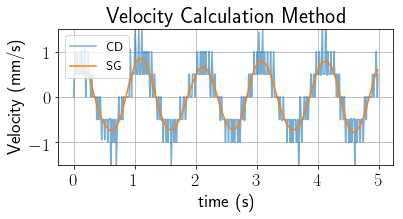
\includegraphics[width=\linewidth]{figs/data/velocity_savgol.png}
    \caption{An illustration of how the Savitky-Golay (SG) filter can be used to calculate the derivative of a signal, and how it compares to the central difference (CD) method.}
    \label{fig:savgol}
\end{figure}

An example of standardized time series voltage and displacement measurements for a measurement run are shown in figure~\ref{fig:correlation}a. The figure demonstrates that the velocity data lags behind the voltage data. The amount of lag can be determined using cross-correlation, which put simply is the sliding inner product of the two series. Cross-correlation is explained further in Appendix~\ref{apx:correlation}.
This time lag is determined to be 120ms in every measurement run conducted for this experiment, with a few outliers at 110ms or 130ms. These measurement runs were conducted with different frequencies, signal amplitudes, and average displacement of the magnet in the coil.
Furthermore it is nonsensical to expect the induced voltage to lead the motion of the magnet. These two points suggest that the time lag is not physical, and is instead a systematic in the data collection process.

\begin{figure}[b]
    \centering
    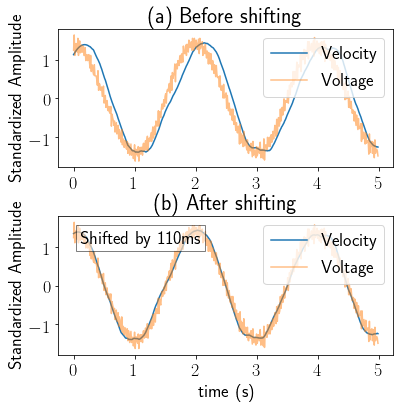
\includegraphics[width=0.85\linewidth]{figs/data/autocorrelation.png}
    \caption{An illustration of how cross-correlation is used to remove a time shift between velocity and voltage signals.}
    \label{fig:correlation}
\end{figure}

One possible explanation is that the RS232 serial interface between the displacement sensor and the LabView program has some fixed overhead that could be contributing to the lag.
Another possible explanation is that the LabView program itself is contributing to the lag in the way it collects the data, averages it, and assigns it to a specific time step.
Further inquiry is needed to determine the exact source of the time shift.

An example of the induced voltage and velocity of a measurement run in the velocity mode is shown in figure~\ref{fig:velocity-example}. The data in this figure was prepared using the methods described above. As the velocity data has been smoothed, the uncertainty in the voltage is assumed to be larger than the uncertainty in the velocity. The uncertainty in the voltage is estimated for each time step as the sample standard deviation within a half wecond window before and after each measurement. For clarity only a 250 point random sample of the full measurement run are shown. The reduced $\chi^2$ value of the fit is 4.21, suggesting the fit is reasonable but some of the uncertainties may be underestimated. The factor $\Phi_v$ can be determined from the slope of this figure using equation~\ref{eq:velocity_equation}. The $\Phi_v$ factor for this example is determined to be $27.325 \pm 0.077\si{Vs/m}$

\begin{figure}[b]
    \centering
    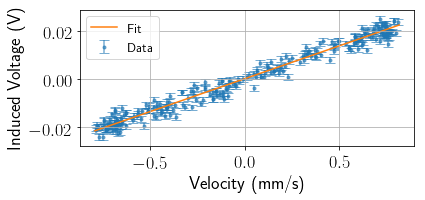
\includegraphics[width=\linewidth]{figs/data/velocity_data_example.png}
    \caption{A sample of velocity and voltage measurements. The process described in this section was used to clean the velocity data. Only a sample of 250 data points are shown for this measurement run.}
    \label{fig:velocity-example}
\end{figure}

The PID setpoint for the force mode measurements was 8.5mm. The center about which the magnets oscillate in the velocity mode can be varied by adding a tare mass to the balance. This experiment assumes that the magnetic field created by the magnets is approximately uniform for small perturbations in the velocity mode. However, as the permanent magnets form a quadrupole, the magnetic field does vary depending on the displacement of the magnets.

\begin{figure}[b]
    \centering
    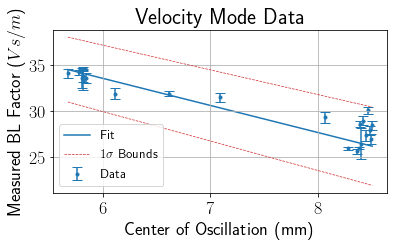
\includegraphics[width=\linewidth]{figs/data/velocity_data.png}
    \caption{Calculated value for $\Phi_v$ as a function of the center of oscillation of the permanent magnet. Many measurements were conducted as described above. The center of oscillation was varied with the tare mass applied to the balance.}
    \label{fig:velocity-data}
\end{figure}

The relationship between $\Phi_v$ and the center of oscillation can be determined by varying the center of oscillation and using the above described method to measure $\Phi_v$. This model can then be used to predict the value of $\Phi_v$ when the balance is oscillating about the 8.5mm displacement used as the setpoint in the force mode measurements. These measurements are shown in figure~\ref{fig:velocity-data}b. The uncertainty in the measurement of $\Phi_v$ for each data point is estimated as the uncertainty in the slope of the linear regression of each fit of voltage and velocity. The weighted residuals for the fit are shown in figure~\ref{fig:velocity-residuals}. The reduced $\chi^2$ value for this model is 16.06. This suggests that the fit is not adequate, and the possibly some of the uncertainties were underestimated. The model predicts a value for $\Phi_v$ as $26.2 \pm 3.0$\si{Vs/m}. The value for $\Phi_v$ differs from $\Phi_f$ by $0.2\sigma$. The error rate of the measurements can be defined as $(\Phi_v-\Phi_f)/\Phi_v$. The error rate for these measurements is 2.4\%.


\begin{figure}[b]
    \centering
    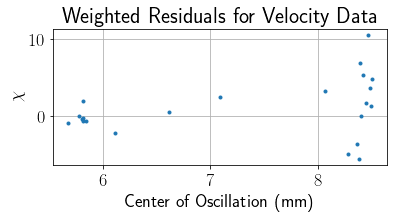
\includegraphics[width=\linewidth]{figs/data/velocity_residuals.png}
    \caption{The weighted residuals for the velocity mode data.}
    \label{fig:velocity-residuals}
\end{figure}


The goal of this experiment was to measure unity between $\Phi_f$ and $\Phi_v$, as expressed in equation~\ref{eq:watt_equation}. The measurements described above yields a value for $\Phi_f/\Phi_v$ of $0.98 \pm 0.11$. Unity is within the margin of error for this value, suggesting the experiment was successful. 


%%%%%%%%%%%%%%%%%%%%%%%%%%%%%%%%%%%%%%%%%%%%%%%%%%%%%%
%%%%%%%%%%%%%%%%%%%%%%%%%%%%%%%%%%%%%%%%%%%%%%%%%%%%%%
\section{CONCLUSION}
%%%%%%%%%%%%%%%%%%%%%%%%%%%%%%%%%%%%%%%%%%%%%%%%%%%%%%
%%%%%%%%%%%%%%%%%%%%%%%%%%%%%%%%%%%%%%%%%%%%%%%%%%%%%%

A Watt balance was built to measure the relationship between mechanical power and electrical power. Such a device could be used to measure the relationship between Planck's constant and the kilogram by using Josephson junctions and quantum resistance standards to measure electrical units in the experiment. The goal of the experiment was to measure unity in $\Phi_f/\Phi_v$, which was measured to be $0.98 \pm 0.11$. However, as the reduced $\chi^2$ value is $>10$ further inquiry may be needed to verify this finding.


 

% \newpage
% \nocite{lab_manual}
% \section{References}


%%%%%%%%%%%%%%%%%%%%%%%%%%%%%%%%%%%%%%%%%%%%%%%%%%%%%%
%%%%%%%%%%%%%%%%%%%%%%%%%%%%%%%%%%%%%%%%%%%%%%%%%%%%%%
\clearpage
\appendix
%%%%%%%%%%%%%%%%%%%%%%%%%%%%%%%%%%%%%%%%%%%%%%%%%%%%%%
%%%%%%%%%%%%%%%%%%%%%%%%%%%%%%%%%%%%%%%%%%%%%%%%%%%%%%
\section{Cross-Correlation}\label{apx:correlation}
In signal processing, cross-correlation is equivalent to the convolution of two signals. The convolution of two discrete signals $f$ and $g$ is defined as
\begin{equation}
    (f*g)[n] = \sum\limits_{m=-\infty}^\infty f[m]\ g[n-m]
    \label{eq:convolution}
\end{equation}
Figure~\ref{fig:correlation_example} illustrates an example of cross-correlation using two phase shifted sine signals. In figure~\ref{fig:correlation_example}a we see two sinusoidal signals, the second having a phase shift of $\pi/8$. Figure~\ref{fig:correlation_example}b shows the output of the cross-correlation function. The maximum correlation appears at $x\approx0.12\pi$. Shifting the data by this amount puts the signals in phase, as shown in figure~\ref{fig:correlation_example}c. 
\newpage

\begin{figure}[h]
    \centering
    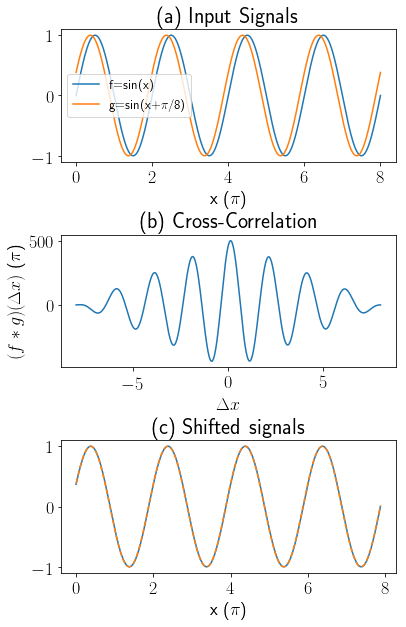
\includegraphics[width=0.9\linewidth]{figs/data/correlation_example.png}
    \caption{An illustration of how cross-correlation can be used to detect how much two time-varying signals have been shifted relative to each other.}
    \label{fig:correlation_example}
\end{figure}



% \onecolumngrid
% \newpage
% \begin{appendices}

% \section{Spectrum Analyzer 14.1.1}\label{apx:block-diagram-14.1.1}

% \appendixpdf{Embedded Microprocessor}{1042_source.pdf}{apx:1042_verilog}
% \end{appendices}


\bibliography{sources.bib}
\end{document}
